\documentclass[11pt,a4paper]{article}

% Define page geometry
\usepackage{geometry} \geometry{left=2.2cm, right=2.2cm, top=2.2cm, bottom=2cm}
\parskip 0.15cm 
\setlength{\parindent}{0cm} 
\usepackage{pdflscape}
\usepackage[document]{ragged2e}

% Text formatting
\usepackage[T1]{fontenc}  % Set font

\usepackage{lineno}  % Line numbers

\usepackage{amssymb}  % Symbols
\usepackage{textcomp}
\newcommand{\textapprox}{\raisebox{0.5ex}{\texttildelow}}  % Command for a good tilde

\linespread{1.5}  % Linespacing

\usepackage{xcolor} \newcommand{\TODO}[1]{\textcolor{red}{\textbf{#1}}}   %

\usepackage{lineno}

% Tables
\usepackage{multirow} \setlength{\tabcolsep}{4pt}

% Image handling
\usepackage{graphicx} 

\makeatletter \g@addto@macro\@floatboxreset\centering  
\makeatother

\graphicspath{ {img/} }  % Define image path

\usepackage{subfig}  % Compound figures

\usepackage{float}  % Precise figure location

% Bibliography management
\usepackage[style=authoryear, natbib=true, backend=biber]{biblatex}
\addbibresource{lidar.bib}

% Links within document, nice figure formatting
\usepackage[breaklinks]{hyperref} \definecolor{links}{RGB}{0,0,0} \hypersetup{
	breaklinks, colorlinks=true, linkcolor=links, anchorcolor=links,
	citecolor=links, filecolor=links, menucolor=links, runcolor=links,
	urlcolor=links, pdfauthor={John L. Godlee} }
	\def\subsectionautorefname{section} \def\subsubsectionautorefname{section}

\newcommand{\beginsupplement}{% 
	\setcounter{table}{0}
	\renewcommand{\thetable}{S\arabic{table}}% 
	\setcounter{figure}{0}
	\renewcommand{\thefigure}{S\arabic{figure}}% 
}
     
% Variables
\newcommand{\rawpt}{2.9e+08}
\newcommand{\voxelpt}{4.5e+07}
\newcommand{\subpt}{2.1e+07}


\newcommand{\titletext}{Species diversity and stand structure as drivers of canopy complexity in southern African woodlands}

\begin{document}

{\LARGE{\titletext{}}}

\linenumbers

\section*{Abstract}

\section{Introduction}

The characterization of tree canopy structure in wooded ecosystems constitutes a long-standing field of research that has been fundamental to interpreting, modelling, and improving understanding of ecosystem function \citep{Watt1947, Whittaker1969, Horn1971, Maarel1996}. Canopy structure describes the spatial distribution and density of canopy foliage, comprising the primary interface between trees, the atmosphere and sunlight. Canopy structural complexity, i.e. the spatial heterogeneity of foliage distribution through the canopy, has been positively linked to canopy productivity \citep{Hardiman2011,Chen2012,Law2001,Baldochii2001,Morin2015}. It is therefore essential to understand the drivers of variation in canopy structure to improve modelling of earth-atmosphere carbon fluxes and community assembly. 

At continental scales, variation in canopy height and canopy cover, two coarse measures of canopy structure both of which have been shown to affect woody productivity and correlate with woody biomass \citep{}, can largely be explained by climate and edaphic data \citep{SOME-GEDI}. Increased resource availability allows for larger trees and more closed canopies \citep{}. At the scale of a single tree community however, where variation in climate and soil may be negligible, variation in canopy structure is thought to be affected principally by an interacting combination of tree canopy species composition \citep{}, and disturbance history \citep{}. However, empirical testing of these mechanisms thought to drive canopy structure in natural wooded ecosystems remains sparse across many biomes \citep{}.

Following established biodiversity-ecosystem function theory, the niche partitioning of canopy space, i.e. the spatial complementarity of individual tree canopies, is thought to be a key mechanism underlying positive biodiversity-productivity effects in wooded ecosystems \citep{Pretzsch2014, Barry2019}. Biodiversity-ecosystem function theory predicts that crown complementarity and thus canopy complexity and foliage density should increase with tree diversity in the local neighbourhood, thus increasing standing biomass and woody productivity, as coexisting species must occupy non-identical niche space to avoid competitive exclusion \citep{Gadow1993}. 

As well as the species diversity of trees in a local neighbourhood, the spatial distribution and relative size dominance of those trees, i.e. stand structure, is also expected to affect crown structural complexity. Increased heterogeneity in tree size, whether a result of species diversity or disturbance history, is expected to increase crown complexity and overall canopy density as individuals of different sizes can occupy different layers of the canopy \citep{}. Additionally, clustering of individuals in space is expected to increase canopy structural heterogeneity across a stand, but ultimately decrease total foliage density due to an increase in competitive interactions \citep{}. Clustering may occur as a result of disturbance history, or as a result of strong facilitation effects among individuals in a hostile environment \citep{Ratcliffe2017}.

While much work in the field of forest management has been done to test biotic drivers of tree canopy structure in temperate \citep{} and boreal forests \citep{}, similar work in the tropics is comparatively scarce \citep{}. In dry tropical woodlands and savannas especially, tree canopy structure and its effect on ecosystem productivity has received little attention, possibly due to the misplaced assumption that woody productivity in these ecosystems does not represent a globally significant carbon flux \citep{}, or that tree canopies in these smaller stature woodlands do not interact and compete for resources to the same degree as in large stature forests \citep{}. In recent years however, it has been shown that dry tropical woodlands represent the largest uncertainty in our estimates of the terrestrial carbon cycle \citep{Quere2018, Ahlstrom2015}. \citet{Sitch2015} demonstrated the dominant role of the dry tropics in driving variability in the terrestrial carbon sink, and showed that the dry tropics are the fastest increasing component of the terrestrial carbon sink. Part of this uncertainty arises from our lacking a nuanced understanding of how species composition and structure affect ecosystem function in these ecosystems, which underpins the Dynamic Global Vegetation Models (DGVMs) fed into global carbon dynamics models. The pertinence of this knowledge gap has prompted further research of the biotic drivers of variation in productivity in the dry tropics, and momentum in this field of research is building \citep{}. 

Canopy structure is multi-dimensional and has previously been explained using a plethora of simple metrics that originated in forest and community ecology \citep{}. Assessments of canopy structure in the dry tropical have most often modelled tree canopies as a series of ellipses (2D) or ellipsoids (3D) based on field measurements with measuring tapes \citep{}. Measurements of this kind are time consuming and yet are an over-simplification of canopy structure \citep{}. Alternatively, canopy cover is often measured using indirect optical methods which partition sky from canopy material, i.e. with hemispherical photography or the commonly used LAI-2000, providing a 2D representation of the canopy but lacking information on vertical canopy structure. In recent years, particularly in temperate and boreal forests, LiDAR (Light Detection And Ranging) has emerged as a suitable technology for rapidly and precisely assessing canopy structure in 3D, conserving information on 3D structure of the calibre that is required to understand it's complexities \citep{}.

In this study we applied terrestrial LiDAR techniques to woodland-savanna mosaics at two sites in southern Africa, with the aim of increasing our understanding of how various metrics of tree canopy structural complexity are affected by tree neighbourhood diversity and stand structure. Our overarching contention is that neighbourhoods of greater tree diversity and greater structural diversity allow greater canopy complexity and foliage density, resulting in higher productivity, and ultimately a more `forest-like' community, rather than an open canopy savanna.

\section{Materials and methods}

\subsection{Study sites}

Measurements were conducted at two sites, the first in Bicuar National Park, southwest Angola (S15.1$^\circ$, E14.8$^\circ$), and the second in and around Mtarure Forest Reserve, southeast Tanzania (S9.0$^\circ$, E39.0$^\circ$) (\autoref{map}). At each site, 1 ha plots were sited in areas of miombo woodland vegetation, across a gradient of stem density. In Angola, 15 plots were sampled, while in Tanzania, seven were sampled following the curtailment of fieldwork due to COVID-19 travel restrictions. Fieldwork was conducted between February and April at both sites, during the peak growth period of each site in order to capture the highest foliage volume in the canopy.

\begin{figure}[H]
\centering
	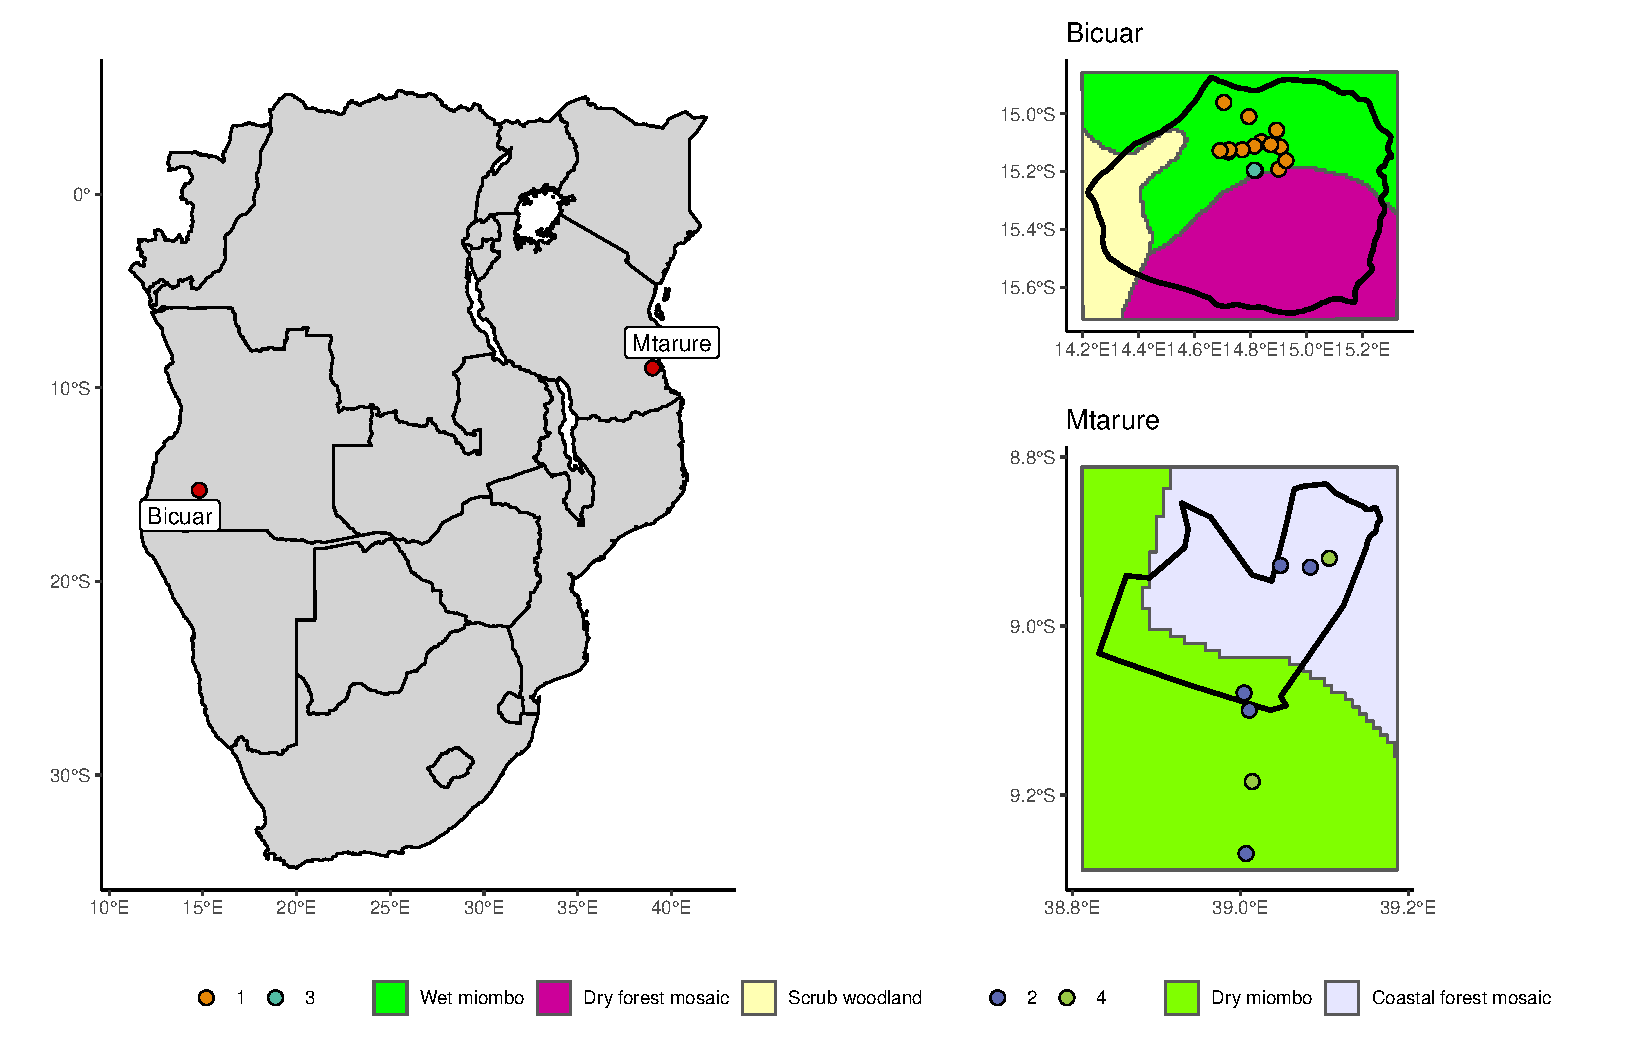
\includegraphics[width=\textwidth]{map}
	\caption{Location of study sites within southern Africa (a), and of 1 ha plots within each site. The blue polygons denote the boundaries of protected areas which encompass the majority of study sites, Bicuar National Park in Angola (b), and Mtarure Forest Reserve in Tanzania (c). The background of each site map is a re-classified version of the GlobCover global land cover classification \citep{Globcover}.}
	\label{map}
\end{figure}

\subsection{Field measurements}

Each plot was further subdivided into nine 10 m diameter circular subplots arranged in a regular grid, with a 15 m buffer from the plot edge and 35 m between subplots. For each subplot, we measured all woody stems >5 cm diameter with canopy material inside the subplot. We identified each stem to species and measured stem diameter (diameter at breast height - 1.3 m), distance and direction of stem from the subplot centre.

Within each subplot, a variable number of scans were recorded using a Leica HDS6100 phase-shift terrestrial laser scanner (TLS) \citep{Leica}. The number and position of scans within a subplot was determined by the arrangement of canopy material in the subplot. Scan positions were arranged to minimise shadows within the canopy of the subplot, and to maximise canopy penetration. The number of scans per subplot ranged between one and five in both sites. 

\subsection{Data analysis}

\subsubsection{Scan processing}

Point clouds from scans in each subplot were registered and unified using Leica Cyclone (version 9.1) \citep{Cyclone}. Targets from each scan were aligned using Cyclone's automatic target acquisition. 

Point clouds were voxelised to cubic voxel sizes of different sizes depending on the application of the data. For subplot height profile estimation and gap fraction we used 5 cm\textsuperscript{3} voxels, and for whole plot canopy rugosity we used 10 cm\textsuperscript{3} voxels. Voxels were classed as filled if they intersected with one or more points. Variation in voxel size reflects the spatial scale of each analysis, and is bounded by the beam divergence of the scanner over longer distances \citep{}. Choosing voxels that are too small can result in pock-marked representations of surfaces that are especially problematic when calculating larger scale canopy structure metrics, such as canopy top roughness, while voxels that are too large can result in an over-estimation of plant volume when estimating canopy foliage density at the subplot scale \citep{Cifuentes2014}. We used a noise reduction algorithm from \citet{} to discard points based on mean nearest neighbour distances. This effectively removed `ghost points' produced by partial interceptions and also removed many erroneous returns caused by airborne dust particles, which was common at our study sites. Raw points clouds for each subplot had \textapprox{}\rawpt{} points, \textapprox{}\voxelpt{} points after voxelisation, and \textapprox{}\subpt{} points after noise reduction.

Ground points were classified using the Progressive Morphological Filter (PMF) from \citet{Zhang2003}. Point cloud height was reclassified height based on this revised ground layer by measuring the vertical distance between the nearest ground point and each point.

We used ray-tracing to calculate canopy cover at the subplot centre from multiple TLS scans. Hemispherical images were created using the POV-ray software \citep{}. Voxels were converted to matt black cubes filling the voxel volume, with a white sky box and no light source. A `camera' with a 180\textdegree{} fisheye lens was placed at the subplot centre within POV-Ray, at a height of 1.8 m pointing directly upwards. The images produced by POV-Ray were analysed using Hemiphot \citep{Steege} to estimate canopy cover as the proportion of pixels filled by canopy material.

\subsection{Stand structure}

For each subplot, we calculated an adapted version of the Hegyi index to estimate crowding, as an alternative to stem density that works better to describe stand structure at small spatial scales \citep{Hegyi1974}. We also calculated the coefficient of variation of stem diameter as a measure of the heterogeneity of tree size in the neighbourhood.

At the plot level, we estimated the regularity of species spatial distribution using the spatial mingling index \citep{Gadow}. We also measured whole plot stand structure using the Winkelmass \citep{}.

\subsection{Statistical analysis}

Linear mixed effects models tested the effects of tree species diversity and stand structure metrics on canopy structure. Two sets of models were conducted, the first at the subplot level with random effects for plot nested within site, and the second at the plot level with random effects for site only. Separate models were fitted for each canopy structure variable, resulting in six models at the subplot level and five models at the plot level.

To explore variation in tree species composition among plots and sites, we conducted a Non-metric Multi-dimensional Scaling (NMDS) analysis using tree species abundance in each plot. We excluded species with only one individual across all plots.  

\section{Results}

\subsection{Vertical canopy complexity}

\begin{figure}[H]
\centering
	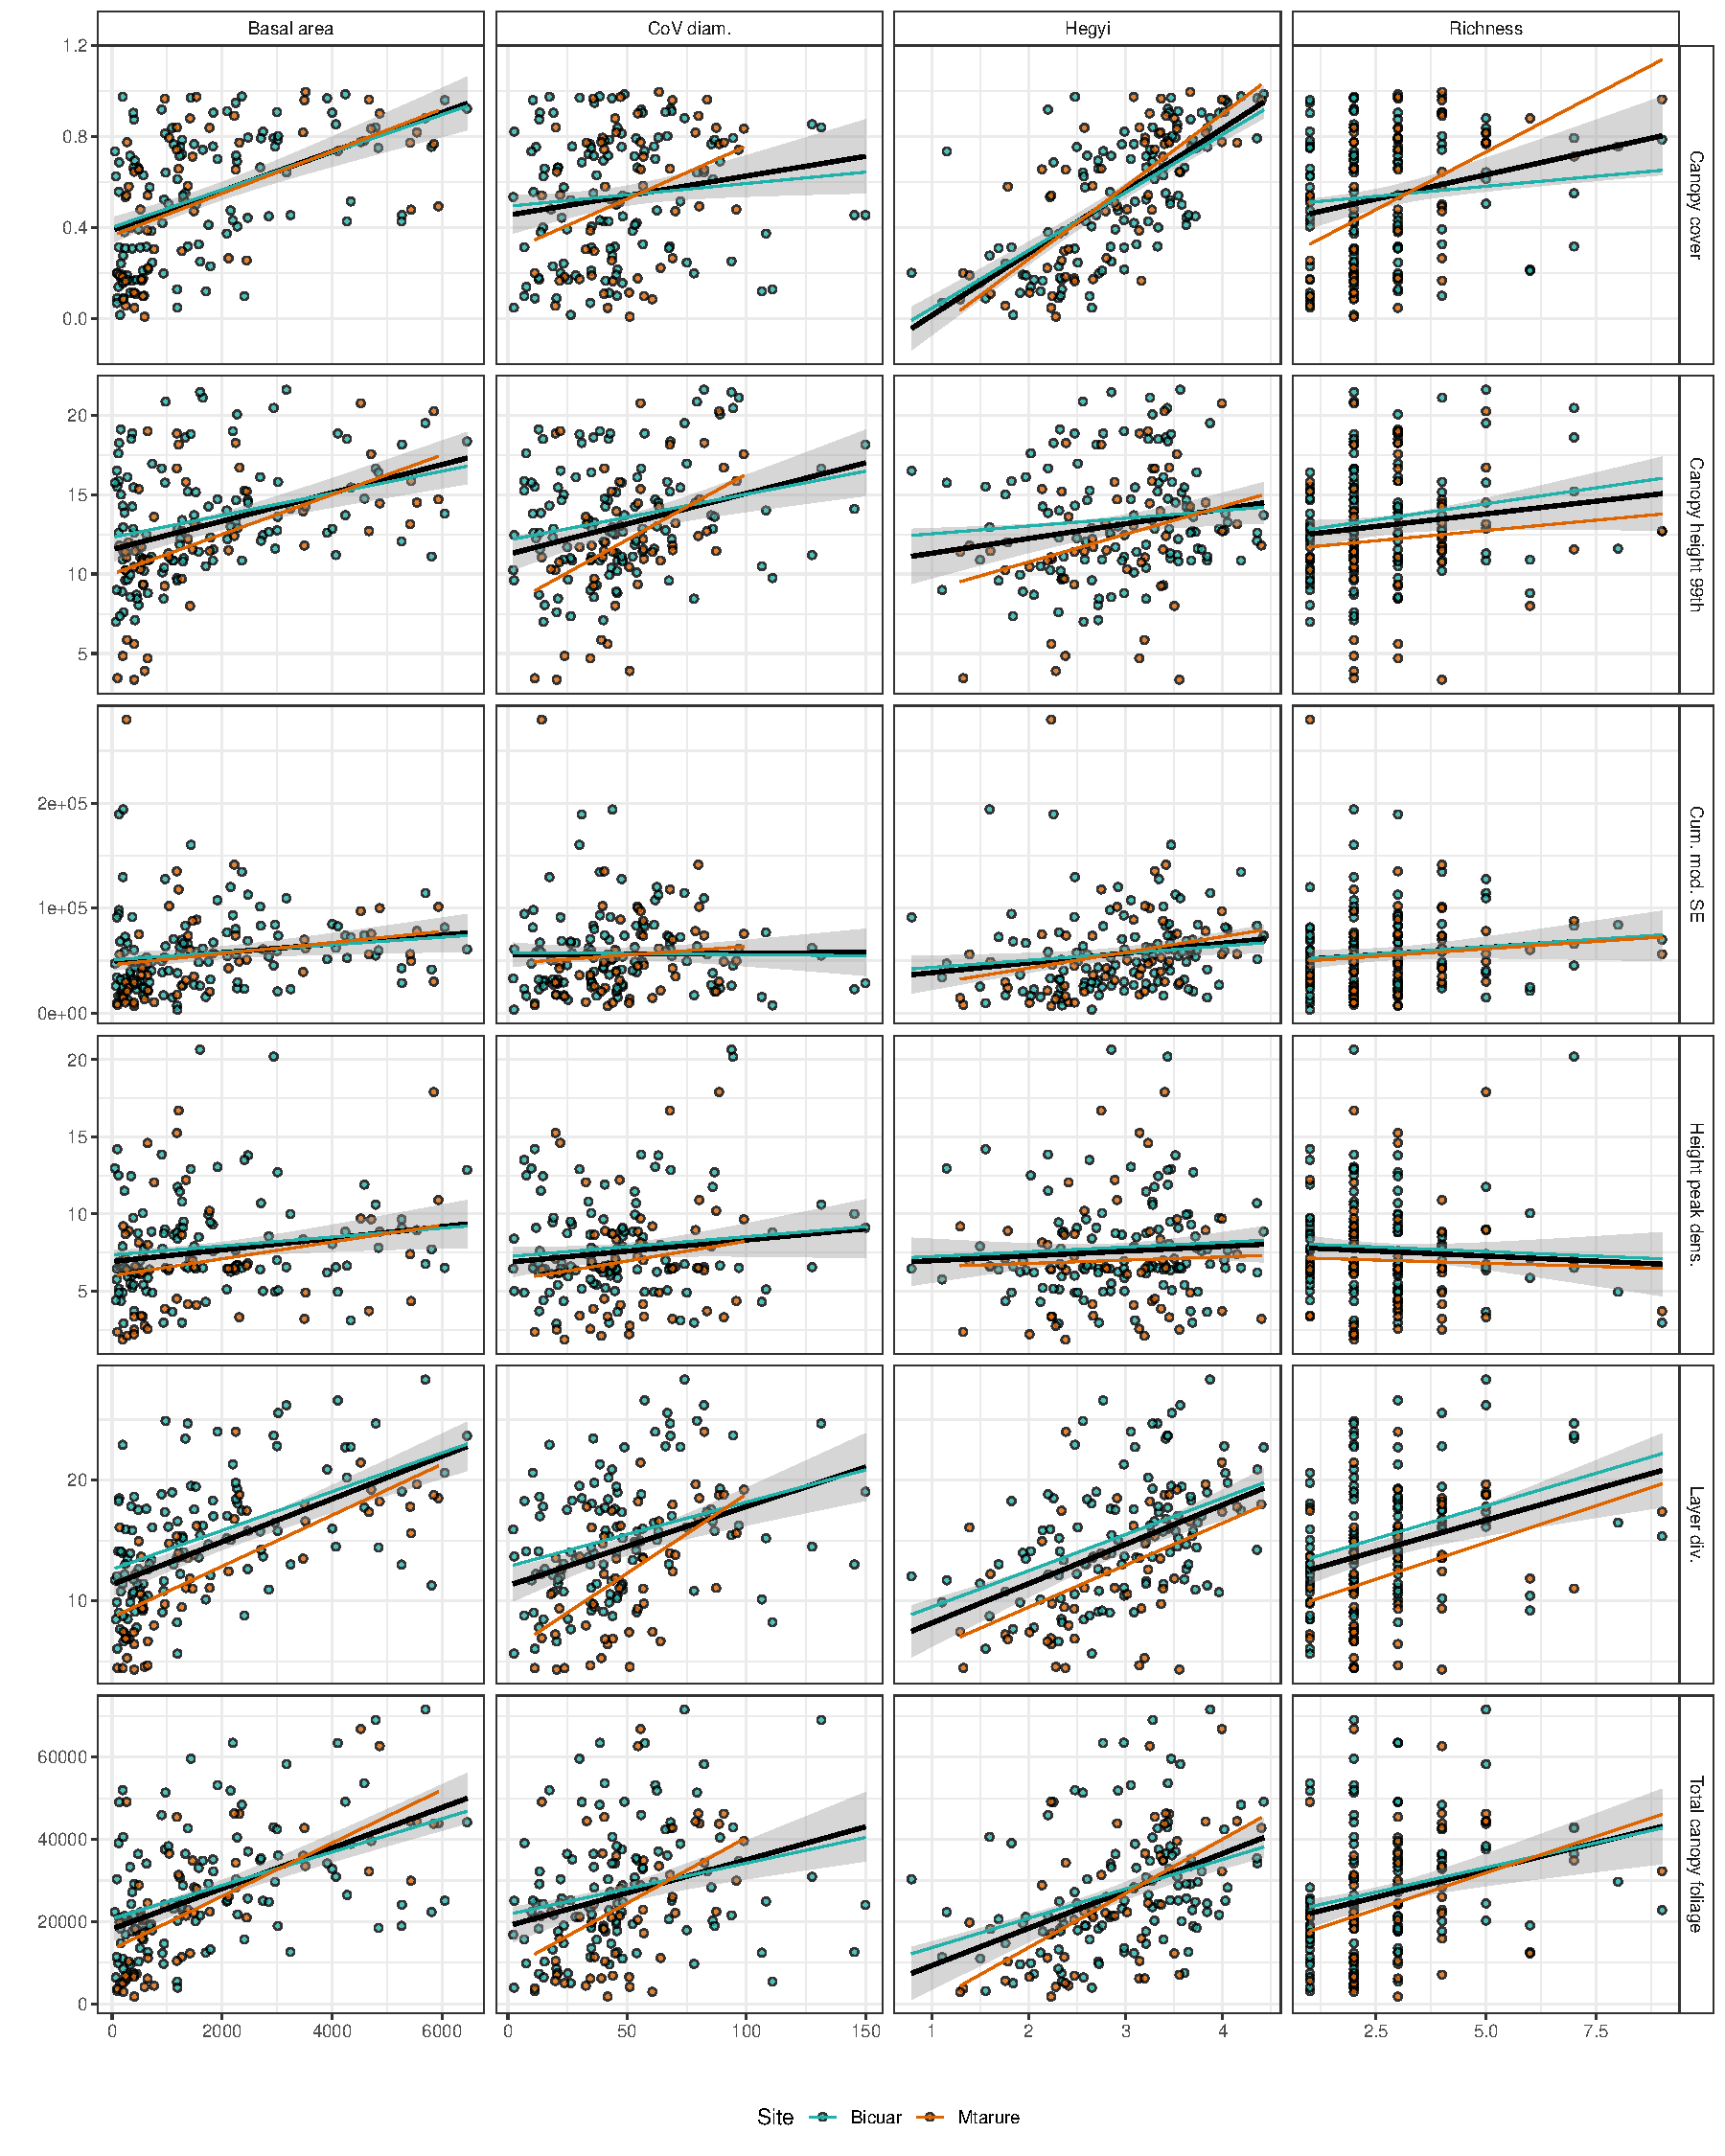
\includegraphics[width=0.8\textwidth]{subplot_canopy_bivar}
	\caption{Bivariate relationships between subplot canopy structure metrics (y axis) and diversity and stand structure metrics (x axis). Points and linear model lines of best fit are coloured by site. The black line of best fit is a linear model including both sites.}
	\label{subplot_canopy_bivar}
\end{figure}

Species diversity, measured by species richness of the tree neighbourhood around each 10 m diameter subplot, appears to have weak but positive effects on canopy layer diversity and total canopy cover, with possibly weak negative effects on the height of peak canopy density. Stand structural metrics have much stronger positive effects on canopy structure, particularly canopy cover and layer diversity. (\autoref{subplot_canopy_bivar}).

Linear mixed effects models showed that species richness of the subplot neighbourhood had variable effects across the measures of canopy structure, but the effect sizes were not significant for any model (\autoref{height_profile_mod_rich_slopes}). On the other hand, stand structural metrics, the Hegyi index, Coefficient of Variation of stem diameter and total stem basal area, had a much greater effect on canopy structure variables. The Hegyi index had a positive significant effect on canopy cover, while basal area had positive significant effects on total foliage density, layer diversity, and canopy height, with strong non-significant effects on non-uniformity of vertical foliage distribution and the height of peak foliage density.

\begin{figure}[H]
\centering
	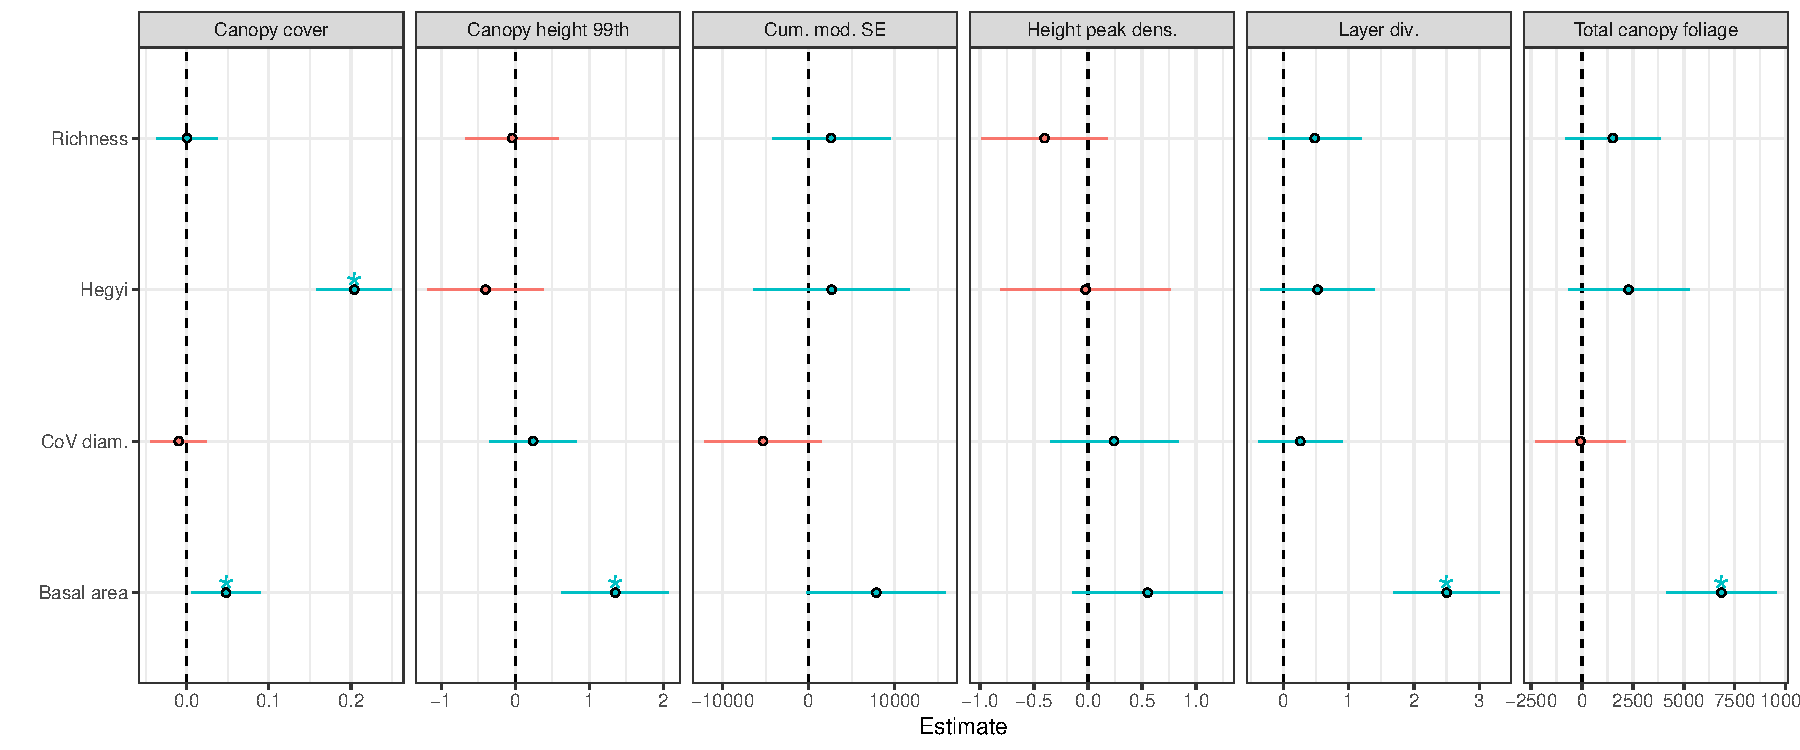
\includegraphics[width=\textwidth]{height_profile_mod_rich_slopes}
	\caption{Standardized fixed effect slopes for each model of a canopy structure metric. Slope estimates are $\pm$1 standard error. Slope estimates where the interval (standard error) does not overlap zero are considered to be significant effects.}
	\label{height_profile_mod_rich_slopes}
\end{figure}

The two sites behaved similarly in mixed models and bivariate linear models.

\subsection{Canopy rugosity}

Similar to the subplot analyses, at the whole-plot scale, tree species diversity tended to have weak positive effects on canopy complexity metrics, while stand structural diversity metrics had stronger positive effects (\autoref{canopy_rough_mod_bivar}). Strong positive relationships of basal area on canopy complexity are driven mostly by two plots with particularly low basal area in Mtarure. These plots are sparse thorny savanna, dominated by \textit{Senegalia} spp. (\autoref{nmds}). Indeed, linear models using only Bicuar plots show divergent relationships. These two plots also have particularly low canopy cover, canopy height, and canopy top roughness, despite having similar tree species richness and spatial distribution of trees (Winkelmass) as other plots.

\begin{figure}[H]
\centering
	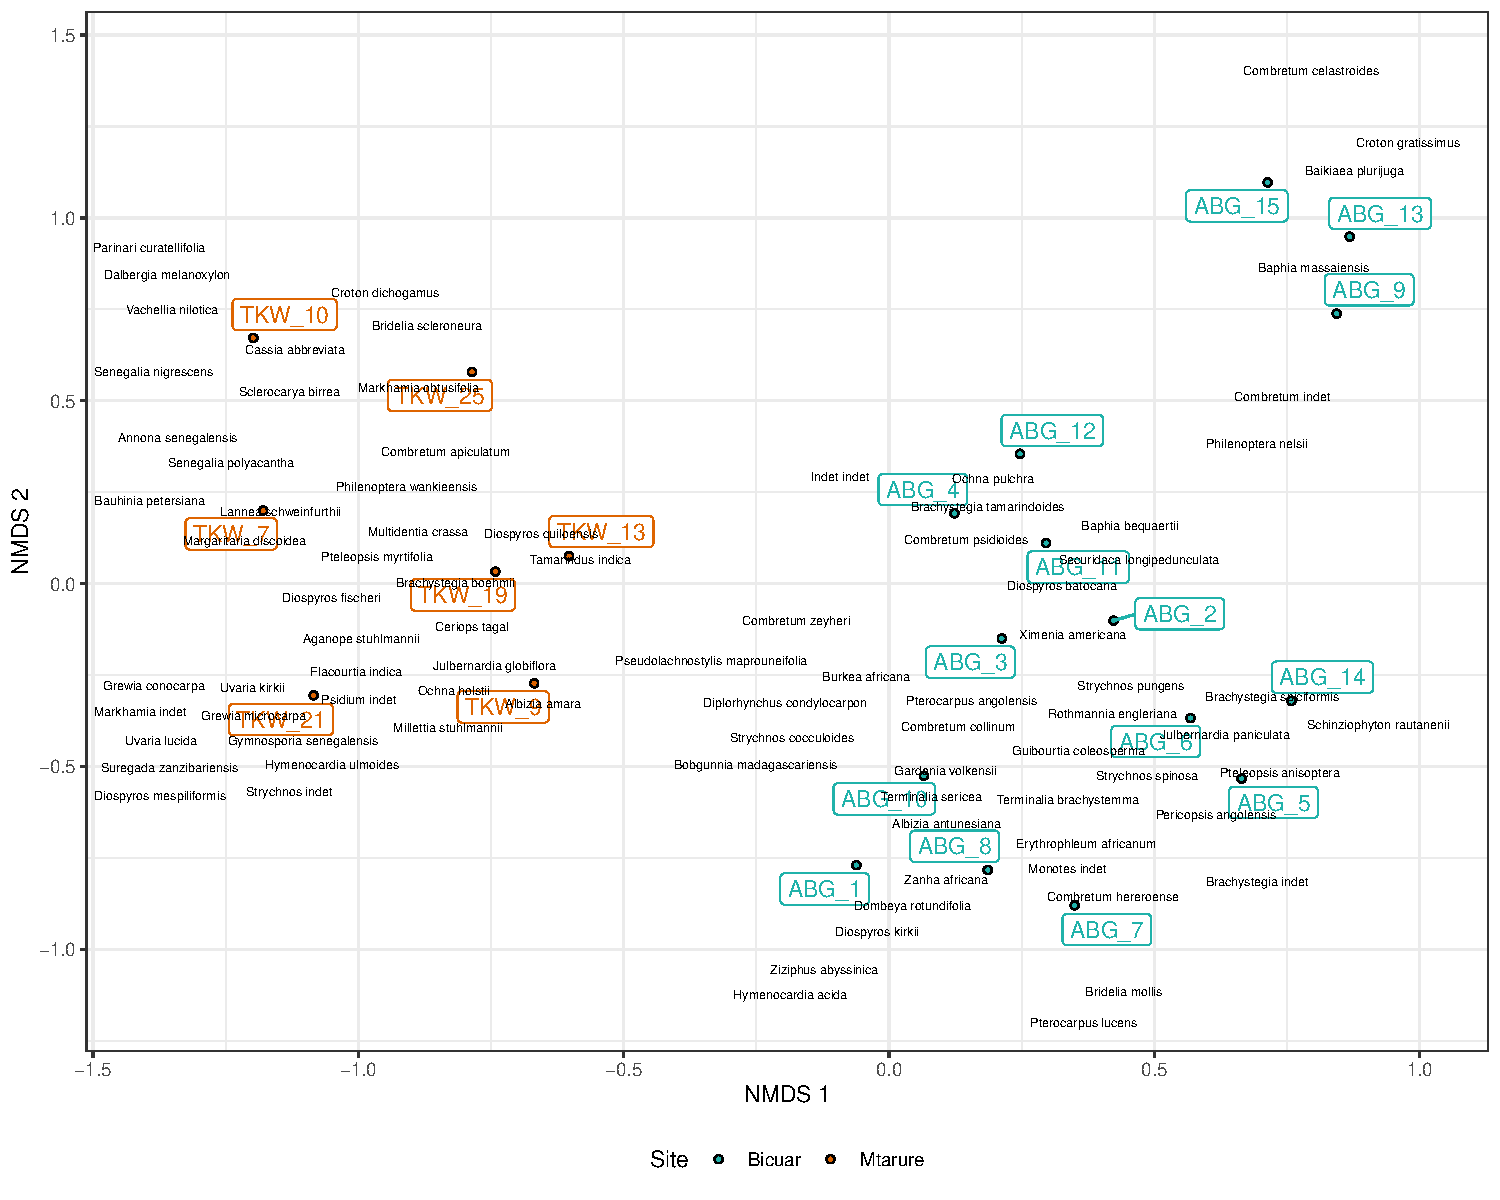
\includegraphics[width=\textwidth]{nmds}
	\caption{The first two axes of a Non-metric Multi-Dimensional Scaling (NMDS) analysis of tree species diversity in each plot. Species scores are labelled as black text, while plot scores are labelled as coloured points. Plots can be split into three principal groups: 1) ABG\_9, ABG\_13 and ABG\_15, dominated by \textit{Baikiaea plurijuga}; 2) the other Bicar plots plus TKW\_9, TKW\_13, TKW\_19 and TKW\_21, dominated by \textit{Julbernardia} spp., \textit{Brachystegia} spp. and \textit{Ochna} spp.; 3) TKW\_7, TKW\_10 and TKW\_25, dominated by \textit{Senegalia} spp. and \textit{Vachellia} spp..}
	\label{nmds}
\end{figure}

\begin{figure}[H]
\centering
	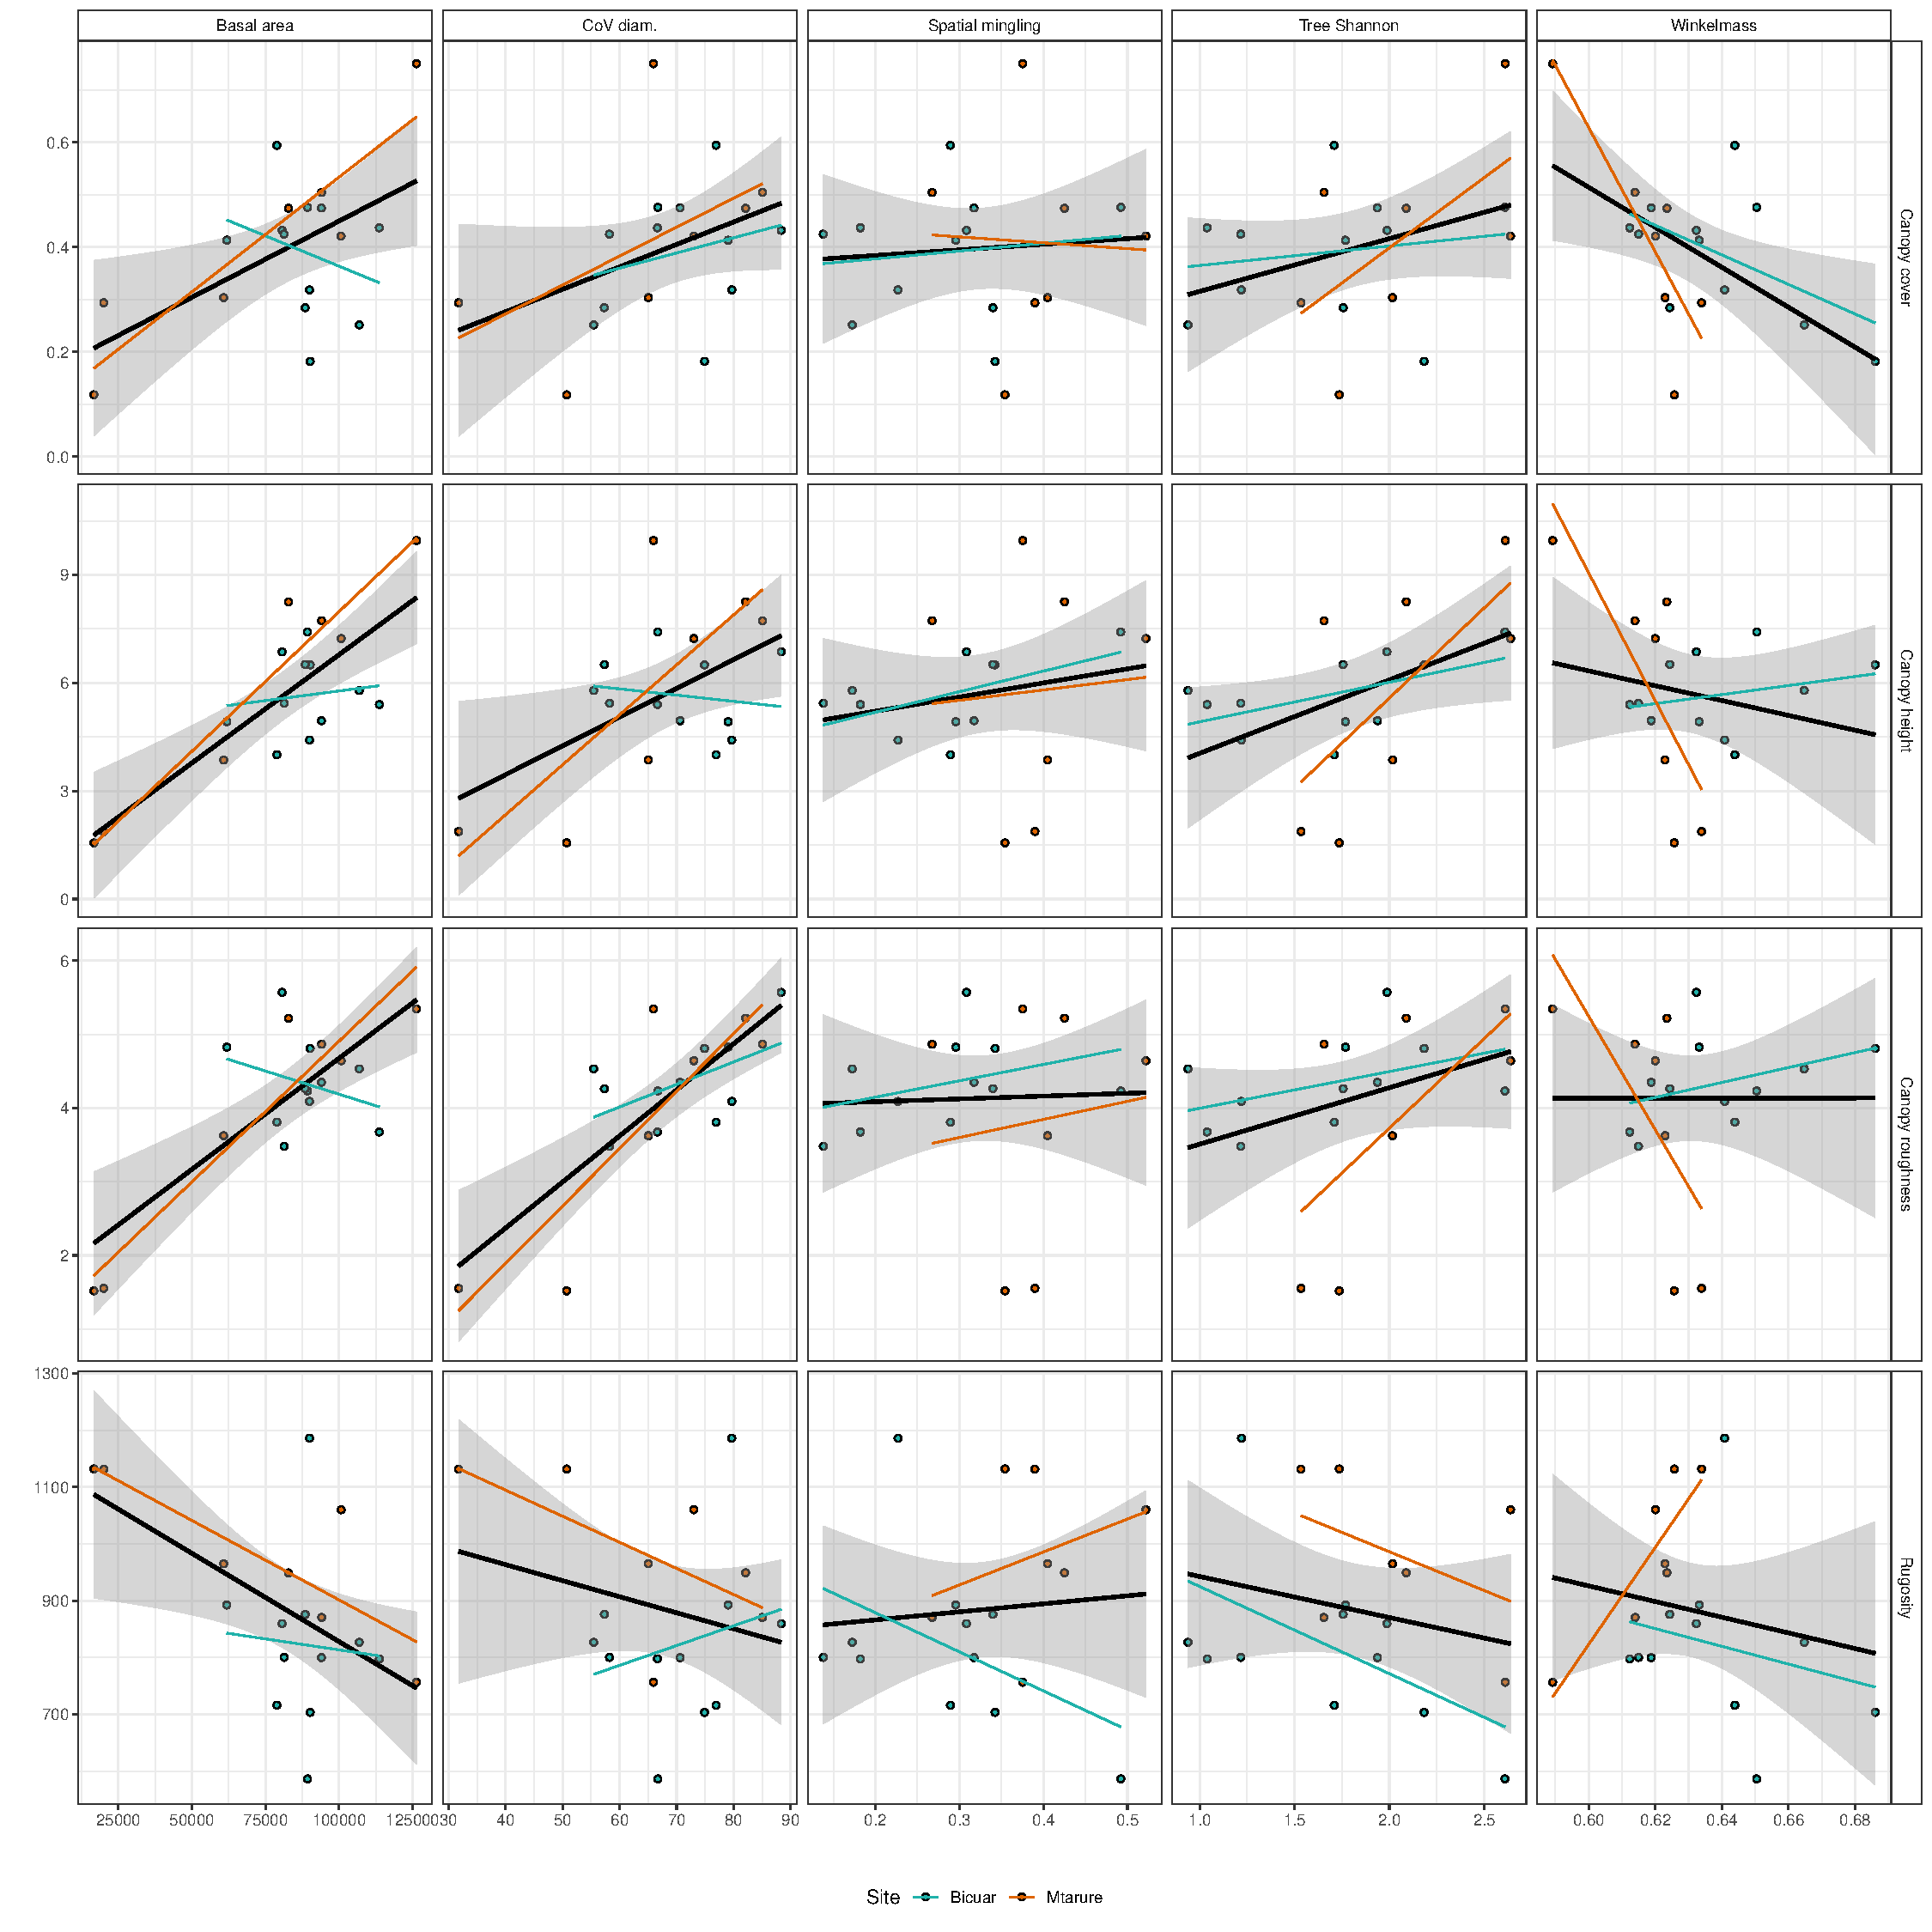
\includegraphics[width=\textwidth]{canopy_rough_mod_bivar}
	\caption{Bivariate relationships between whole-plot canopy structure metrics (y axis) and diversiy and stand structure metrics (x axis). Points and linear model lines of best fit are coloured by site. The black line of best fit is a linear model including both sites.}
	\label{canopy_rough_mod_bivar}
\end{figure}

Maximum canopy height at the plot-level appears to be positively affected by both tree species diversity and total stem basal area. Basal area has a positive effect on canopy top roughness. Variation in canopy height was increased both by variation in stem diameter and total stem basal area. The only significant fixed effect on canopy cover at the plot level was the Winkelmass, which measures the spatial clustering of trees.

\begin{figure}[H]
\centering
	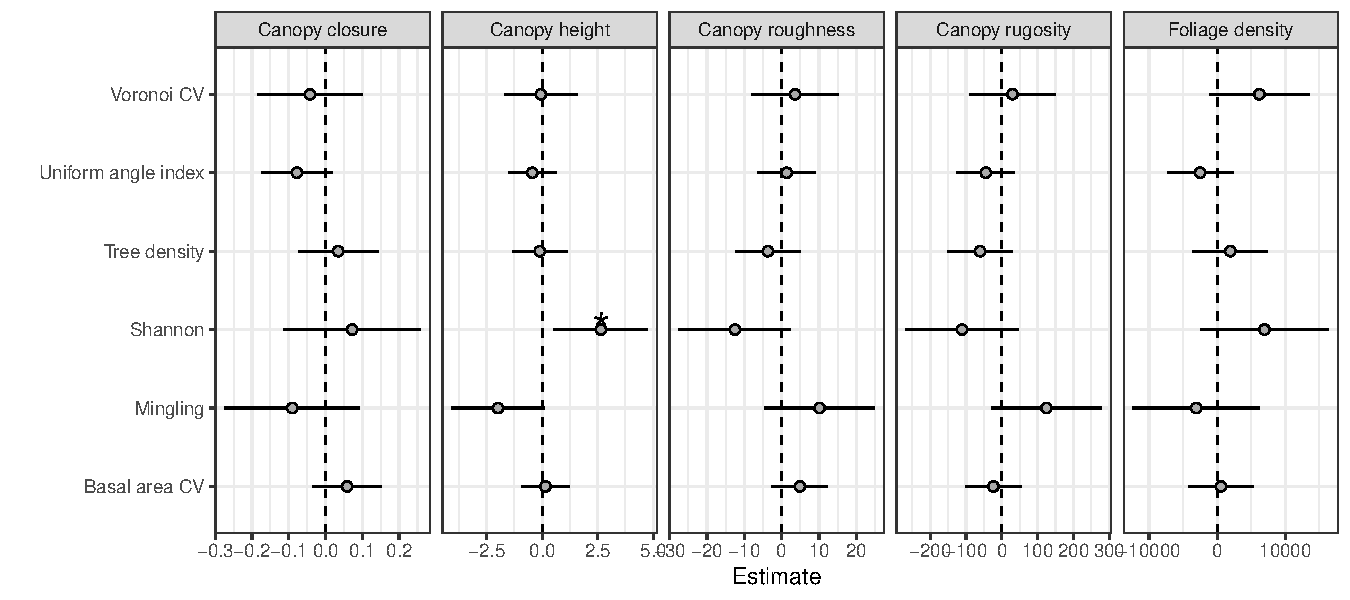
\includegraphics[width=\textwidth]{canopy_rough_slopes}
	\caption{Standardized fixed effect slopes for whole-plot canopy rugosity. Slope estimates are $\pm$1 standard error. Slope estimates where the interval (standard error) does not overlap zero are considered to be significant effects.}
	\label{canopy_rough_slopes}
\end{figure}

\subsection{Comparing subplot and plot measures of canopy structure}

Plot-level and subplot-level canopy structure metrics were highly correlated in many cases (\autoref{canopy_rough_slopes}). Notably, as canopy top rugosity increases, various subplot canopy complexity and density metrics decrease. Additionally, as canopy top roughness increases, many subplot canopy complexity and density metrics increase.


\begin{figure}[H]
\centering
	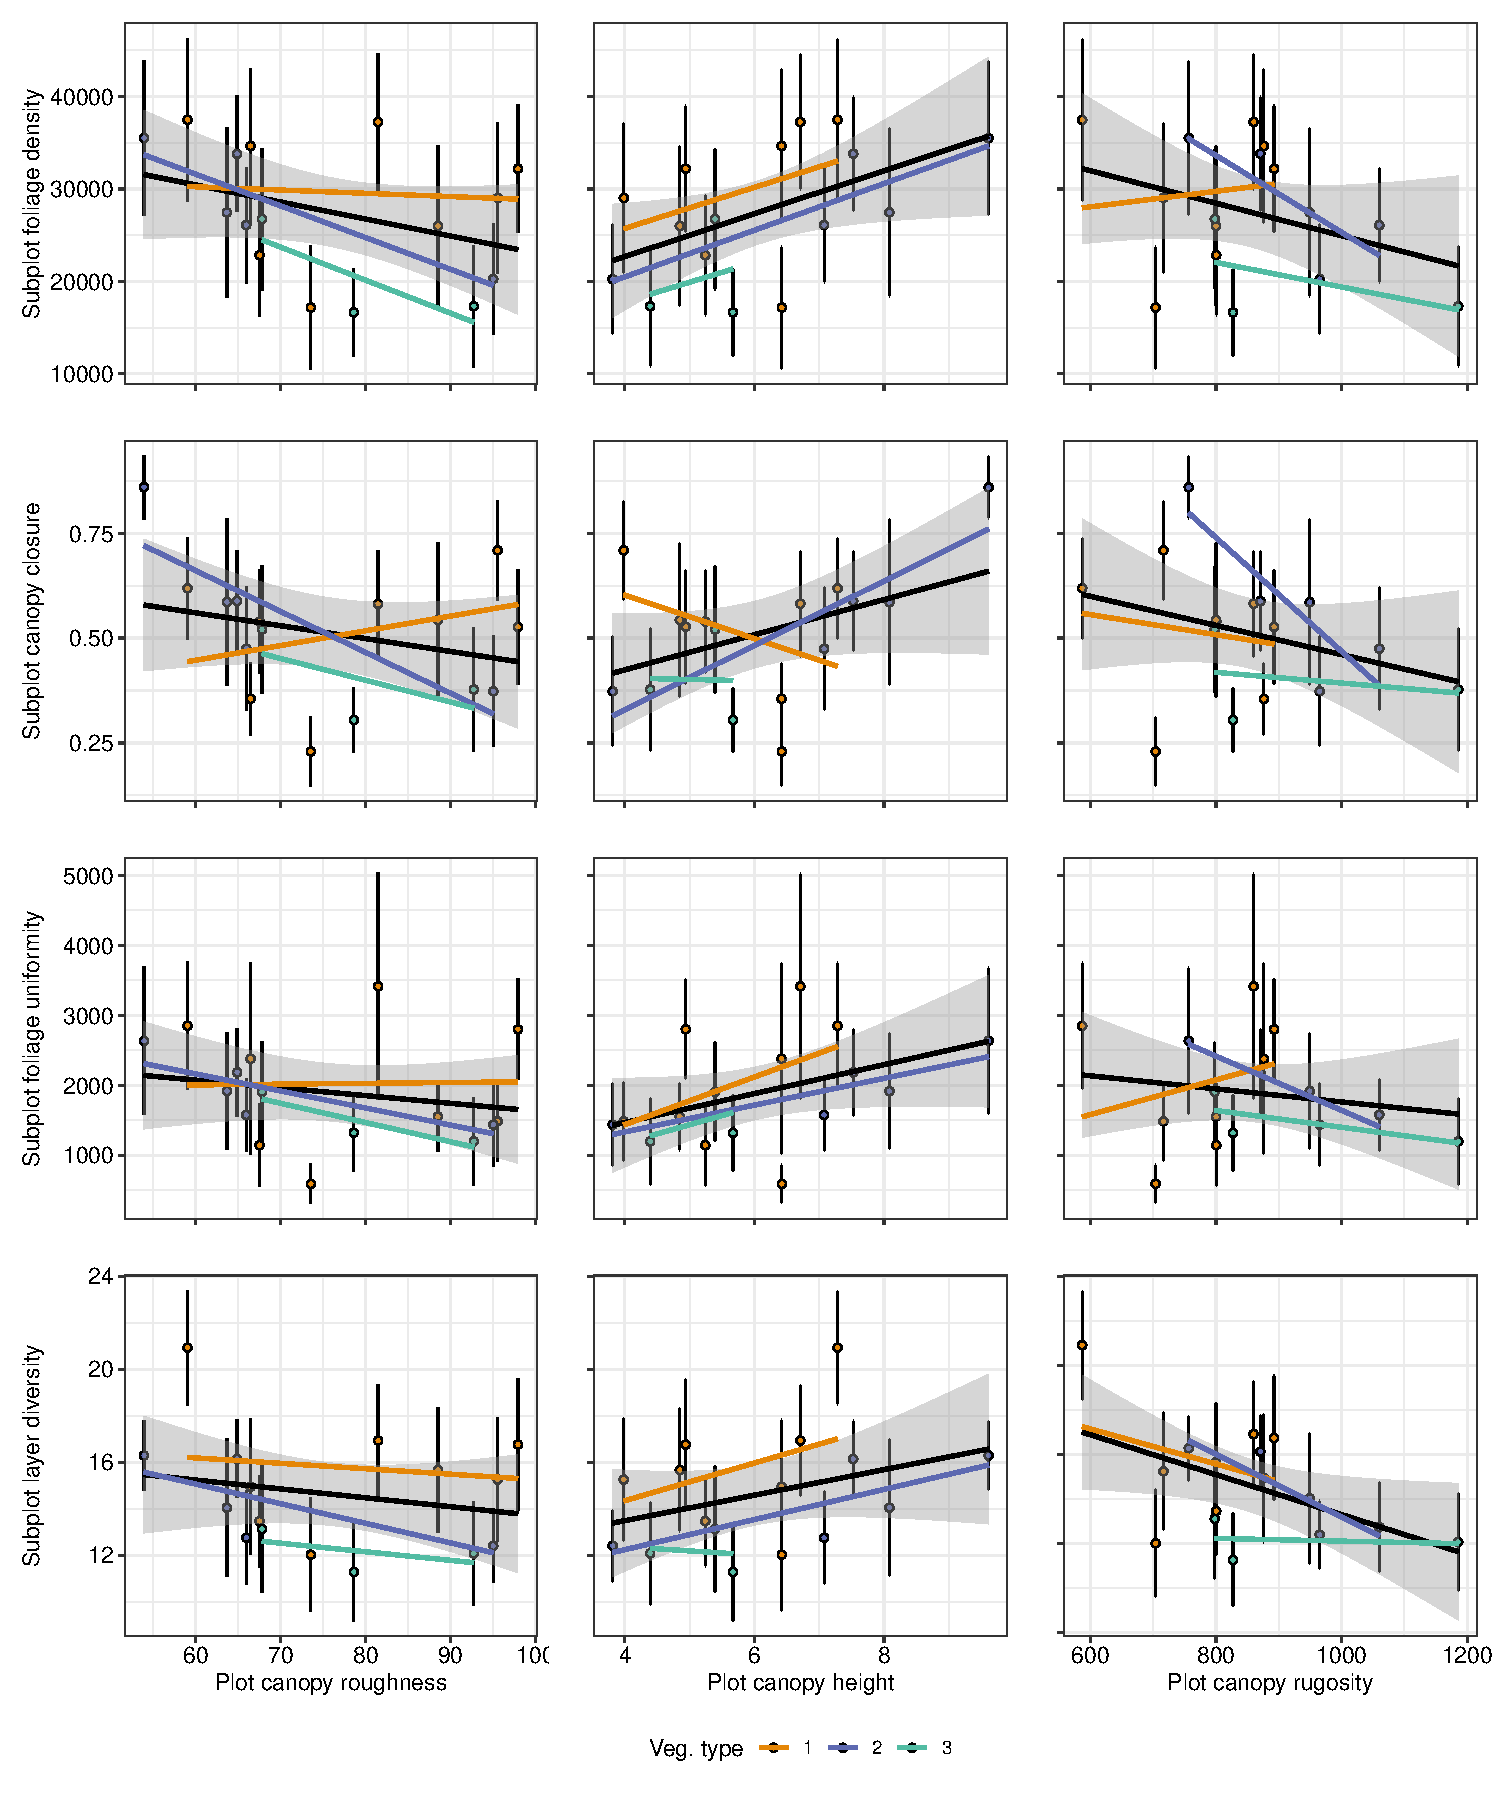
\includegraphics[width=\textwidth]{plot_subplot_bivar}
	\caption{Bivariate plots of canopy structural metrics at the subplot and plot-level. Each point represents the mean values of a single plot. Points and linear model fits are coloured according to site. The black linear model combines both sites. Error bars on points are the standard deviation of subplot metrics.}
	\label{plot_subplot_bivar}
\end{figure}



\section{Discussion}

We investigated the effects of tree species diversity and structural diversity on several metrics of canopy structure that are hypothesised to affect plot productivity. Species diversity appeared to have weak positive effects on canopy complexity at both the subplot and plot scales, while stand structural diversity had greater effects.

With the whole plot effect of tree species diversity on canopy height, what we might be seeing is actually an increased canopy height allowing greater species diversity, rather than the other way round.

While there are reasons to think that stand structure would influence species diversity directly, we did not find evidence for this in our study. Correlations between CoV stem diameter and richness were weak \TODO{check}.


\citet{Jucker2015} found that increased species diversity led to greater canopy packing in European forests, with trees in mixed forests having generally larger crowns. Our result that species richness correlated with greater canopy cover and canopy complexity supports this, though mixed models suggest that the role of richness is heavily tempered by stand structure and the spatial distribution of individuals. In disturbed woodlands, disturbance appears to be the primary determinant of canopy complexity, while species richness plays a supporting role.

\section{Conclusion}

\printbibliography

%\section{Supplementary Material} \beginsupplement

\end{document}
